\section{Test}

Det er meget vigtigt at have et robust kontrol system, der er skræddersyet til vores system. Derfor er det stærkt nødvendigt at teste vores system på alle de punkter, der kan have inflydelse på denne. Der er en lang række faktorer, der skal være med i modellen, for at kontrol systemet kan opfører sig som forventet. Den simpleste metode at tage højde for disse, er at måle deres inflydelse, og så eventuelt justere dem hvis dette er muligt.

\subsection{Step Respons Tilt}

For at lave en grey box model af motoren, skal step responsen for omdrejningerne i forhold til spændingen over motorterminalerne findes. Det vil, med andre ord, sige at ændringen i motoromdrejningerne over tid skal måles ved en konstant spænding. Da motoren allerede er udstyret med en encoder, er det muligt at måle omdrejningshastigheden fra de to hall sensorer ved hjælp af en logic analyzer. Denne analyzer gør det muligt, at se hvor lang tid der går imellem flankerne på pulserne fra hall sensorerne, og på den måde udregne vinkelhastigheden derfra. 
Hver hall sensor giver 3 pulser på en omgang - det svarer til $2\pi/6$ radianer fra en rising edge til en falling edge og omvendt. Logic analyzeren tilsluttes de to hall sensorer, og måler motorens respons i det øjeblik en konstant spænding på 12V sættes over motorterminalerne. Testen udføres 5 gange for at kunne sammenligne resultaterne. 

Hall-sensorerne Når målingerne fra hall-sensorerne er regnet om til $rad/s$ og slået sammen til ét plot, produceres et plot der er meget støjet. Ud fra plottet på figur \ref{fig:Ubehandlet} kan man se at støjen er periodisk - det skyldes primært to faktorer: Hvis hall sensorerne ikke sidder præcist 90 grader forskudt, vil afstanden imellem flankerne på signalet heller ikke altid passe med $2\pi/6$ radianer, som det er antaget i udregningen af vinkelhastigheden. Det vil resultere i hastigheder, der er enten for høje eller for lave i forhold til virkeligheden - denne fejl vil gentage sig periodisk fordi afvigelsen fra $2\pi/6$ radianer vil være den samme altid. Den anden faktor, der har samme effekt på plottet, er polerne i rotoren - de vil heller aldrig være forskudt med helt den samme vinkel.

\begin{figure}[!ht]
	\begin{center}
		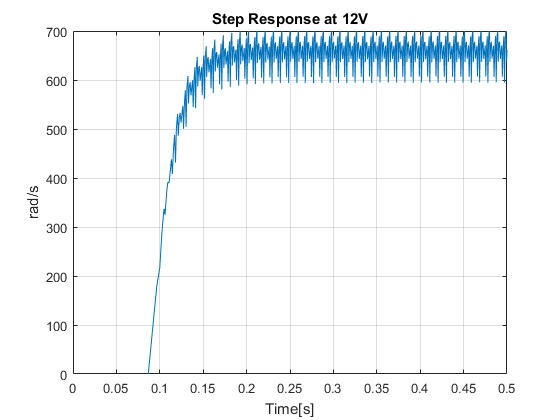
\includegraphics[width=0.8\textwidth]{Billeder/Untreated_Response.png}
	\end{center}
\caption{Den målte step respons i rad/s ved 12V konstant spænding. Omdrejningshastigheden er beregnet ud fra tiden imellem flankerne på hall sensor-signalerne. Der er extrapoleret ned til 0 rad/s ud fra hældningen på de første to målinger.}
\label{fig:Ubehandlet}
\end{figure}

Hvis man nærstuderer figur \ref{fig:Ubehandlet}, kan man se at udsvingene gentager sig selv hver 12. sample. Det passer perfekt med at hver hall sensor har 6 halvperioder, hvor der bliver målt en tid, pr omgang. Det er med andre ord muligt at justere for fejlen ved at gange en faktor på alle samples, der tager højde for afvigelsen fra de $2\pi/6$ radianer. I matlab kan man relativt simpelt finde de 12 faktorer, ved at undersøge hvor meget 12 konsekutive samples afviger fra gennemsnittet, så længe det bliver gjort i et område hvor responsen har nået steady state. Så er det bare et spørgsmål om at gange faktorerne på alle samples med det rette offset for at justere for fejlen. 

\begin{figure}[!ht]
	\begin{center}
		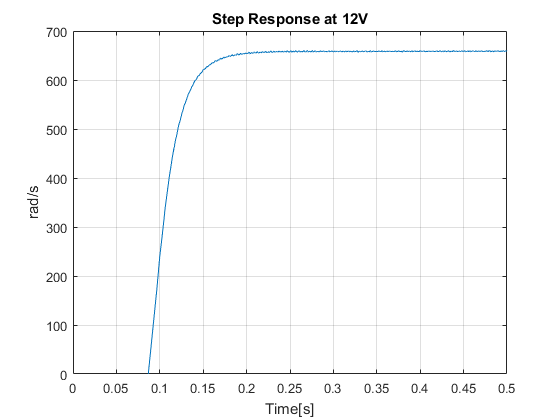
\includegraphics[width=0.8\textwidth]{Billeder/Treated_Response.png}
	\end{center}
\caption{Den målte step respons justeret for periodiske fejl.}
\label{fig:Behandlet}
\end{figure}

På det nye plot det noget lettere at aflæse tidskonstanten for systemet. Den eneste store usikkerhed der er tilbage er starttidspunktet for steppet, da det ikke indgår i målingerne fra logic analyzeren - det er en tilnærmet værdi ud fra hældningen af de første par samples ($\Delta\omega/\Delta t$). Plottene på figur \ref{fig:Ubehandlet} og \ref{fig:Behandlet} viser responsen for motoren uden belastning. Den aflæste tidskonstant på figur \ref{fig:Behandlet} er 27.3 ms.

Samme metode kan bruges til at måle step-responsen for motoren med belastning, så man kan få et billede af hvilken effekt den ekstra modstand har på systemet. På figur \ref{fig:Combined} kan man se responsen for motoren uden belastning (blå), motoren kun med tilt-rammen (rød), motoren med tilt-rammen og kamerabeslag (gul) og motoren med tilt-rammen, beslag og kamera monteret (lilla). Det er tydeligt at rammernes afbalancering har en stor indflydelse på responsen.

\begin{figure}[!ht]
	\begin{center}
		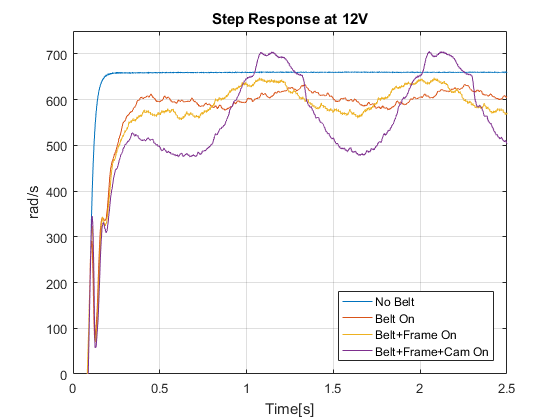
\includegraphics[width=0.8\textwidth]{Billeder/Response_Combined.png}
	\end{center}
	\caption{Step Respons for tilt-motoren uden belastning (blå); med rammen monteret (rød); med rammen og beslaget monteret (gul); og med rammen, beslaget og kameraet (lilla).}
	\label{fig:Combined}
\end{figure}

Det kan også ses, at responsen for motoren, når den er forbundet med rammen, følger responsen for motoren uden belastning det første korte stykke tid, hvorefter hastigheden falder markant. En forklaring kunne være slør i forbindelsen mellem motoren og rammen - i den situation kan den fysiske modstand fra rammen først mærkes af motoren, når bælterne er blevet trukket helt i spænd. En anden ting der også er tydelig er, at selv når der ikke er monteret ekstra udstyr på rammen, så er der stadig en ubalance i rammen, der får hastigheden til at være ujævn over en hel omgang.

Det er stadigvæk muligt at approksimere systemet som et 1.-ordenssystem, men modellen vil udelukkende beskrive, hvor hurtigt systemet reagerer på inputs og ikke så meget om den præcise opførsel. Det vil dog være en rigtig god ide, at få afbalanceret rammerne så godt som muligt og gøre modstanden nogenlunde konstant over en hel omgang, for at modellen kan afspejle virkeligheden så godt som muligt. Med rammen forbundet med motoren er tidskonstanten omkring 125 ms.

\subsection{Step Respons Pan}

Step responsen for pan-systemet kan findes ud fra samme fremgangsmåde som blev benyttet på tilt-systemet. Der er dog den begrænsning, at pan-systemet ikke kan dreje ret meget mere end en halv omgang før ledningerne til tilt-systemet bliver spændt ud. Dette gør det svært at finde systemets steady state værdi og i forlængelse deraf også tidskonstanten. Det kan lade sig gøre at estimere steady state-værdien nogenlunde ud fra et ufuldstændigt plot, men præcisionen vil ikke være så stor som den var for tilt-systemet. 

I forhold til tilt-systemet forventes det at tidskonstanten er noget større, da pan-systemet bærer vægten fra begge systemer - dette vil resultere i et større inertimoment. 

\begin{figure}[!ht]
	\begin{center}
		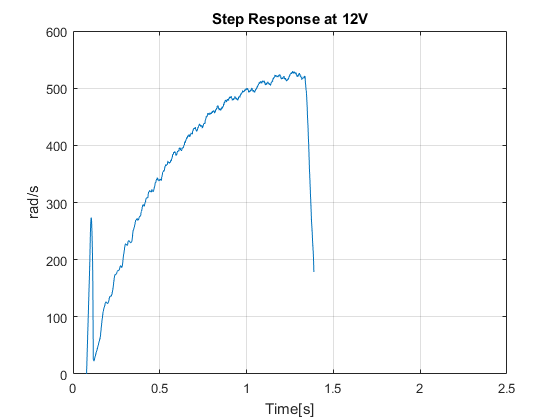
\includegraphics[width=0.8\textwidth]{Billeder/Pan_Response.png}
	\end{center}
	\caption{Step Respons for pan-rammen med kamera monteret}
	\label{fig:Pan_Response}
\end{figure}

Det kan ses på figur \ref{fig:Pan_Response} at responsen er noget langsommere, ligesom at den endelige omdrejningshastiged, på ca 530 rad/s, også er omkring 100 rad/s langsommere end for tilt-systemet. Den aflæste tidskonstant for pan-systemet fås til at være ca. 440 ms.

\subsection{Afbalancering}

Der blev erfaret at det var svært at placere det påmonterede kamera så tilt delen af systemet var i balance. Der blev besluttede at prøve at afbalancere systemet ved at tilføje vægt. På figur \ref{fig:Afbalancering} kan man se den tilføjede vægt på systemet

\begin{figure}[!hb]
	\begin{center}
		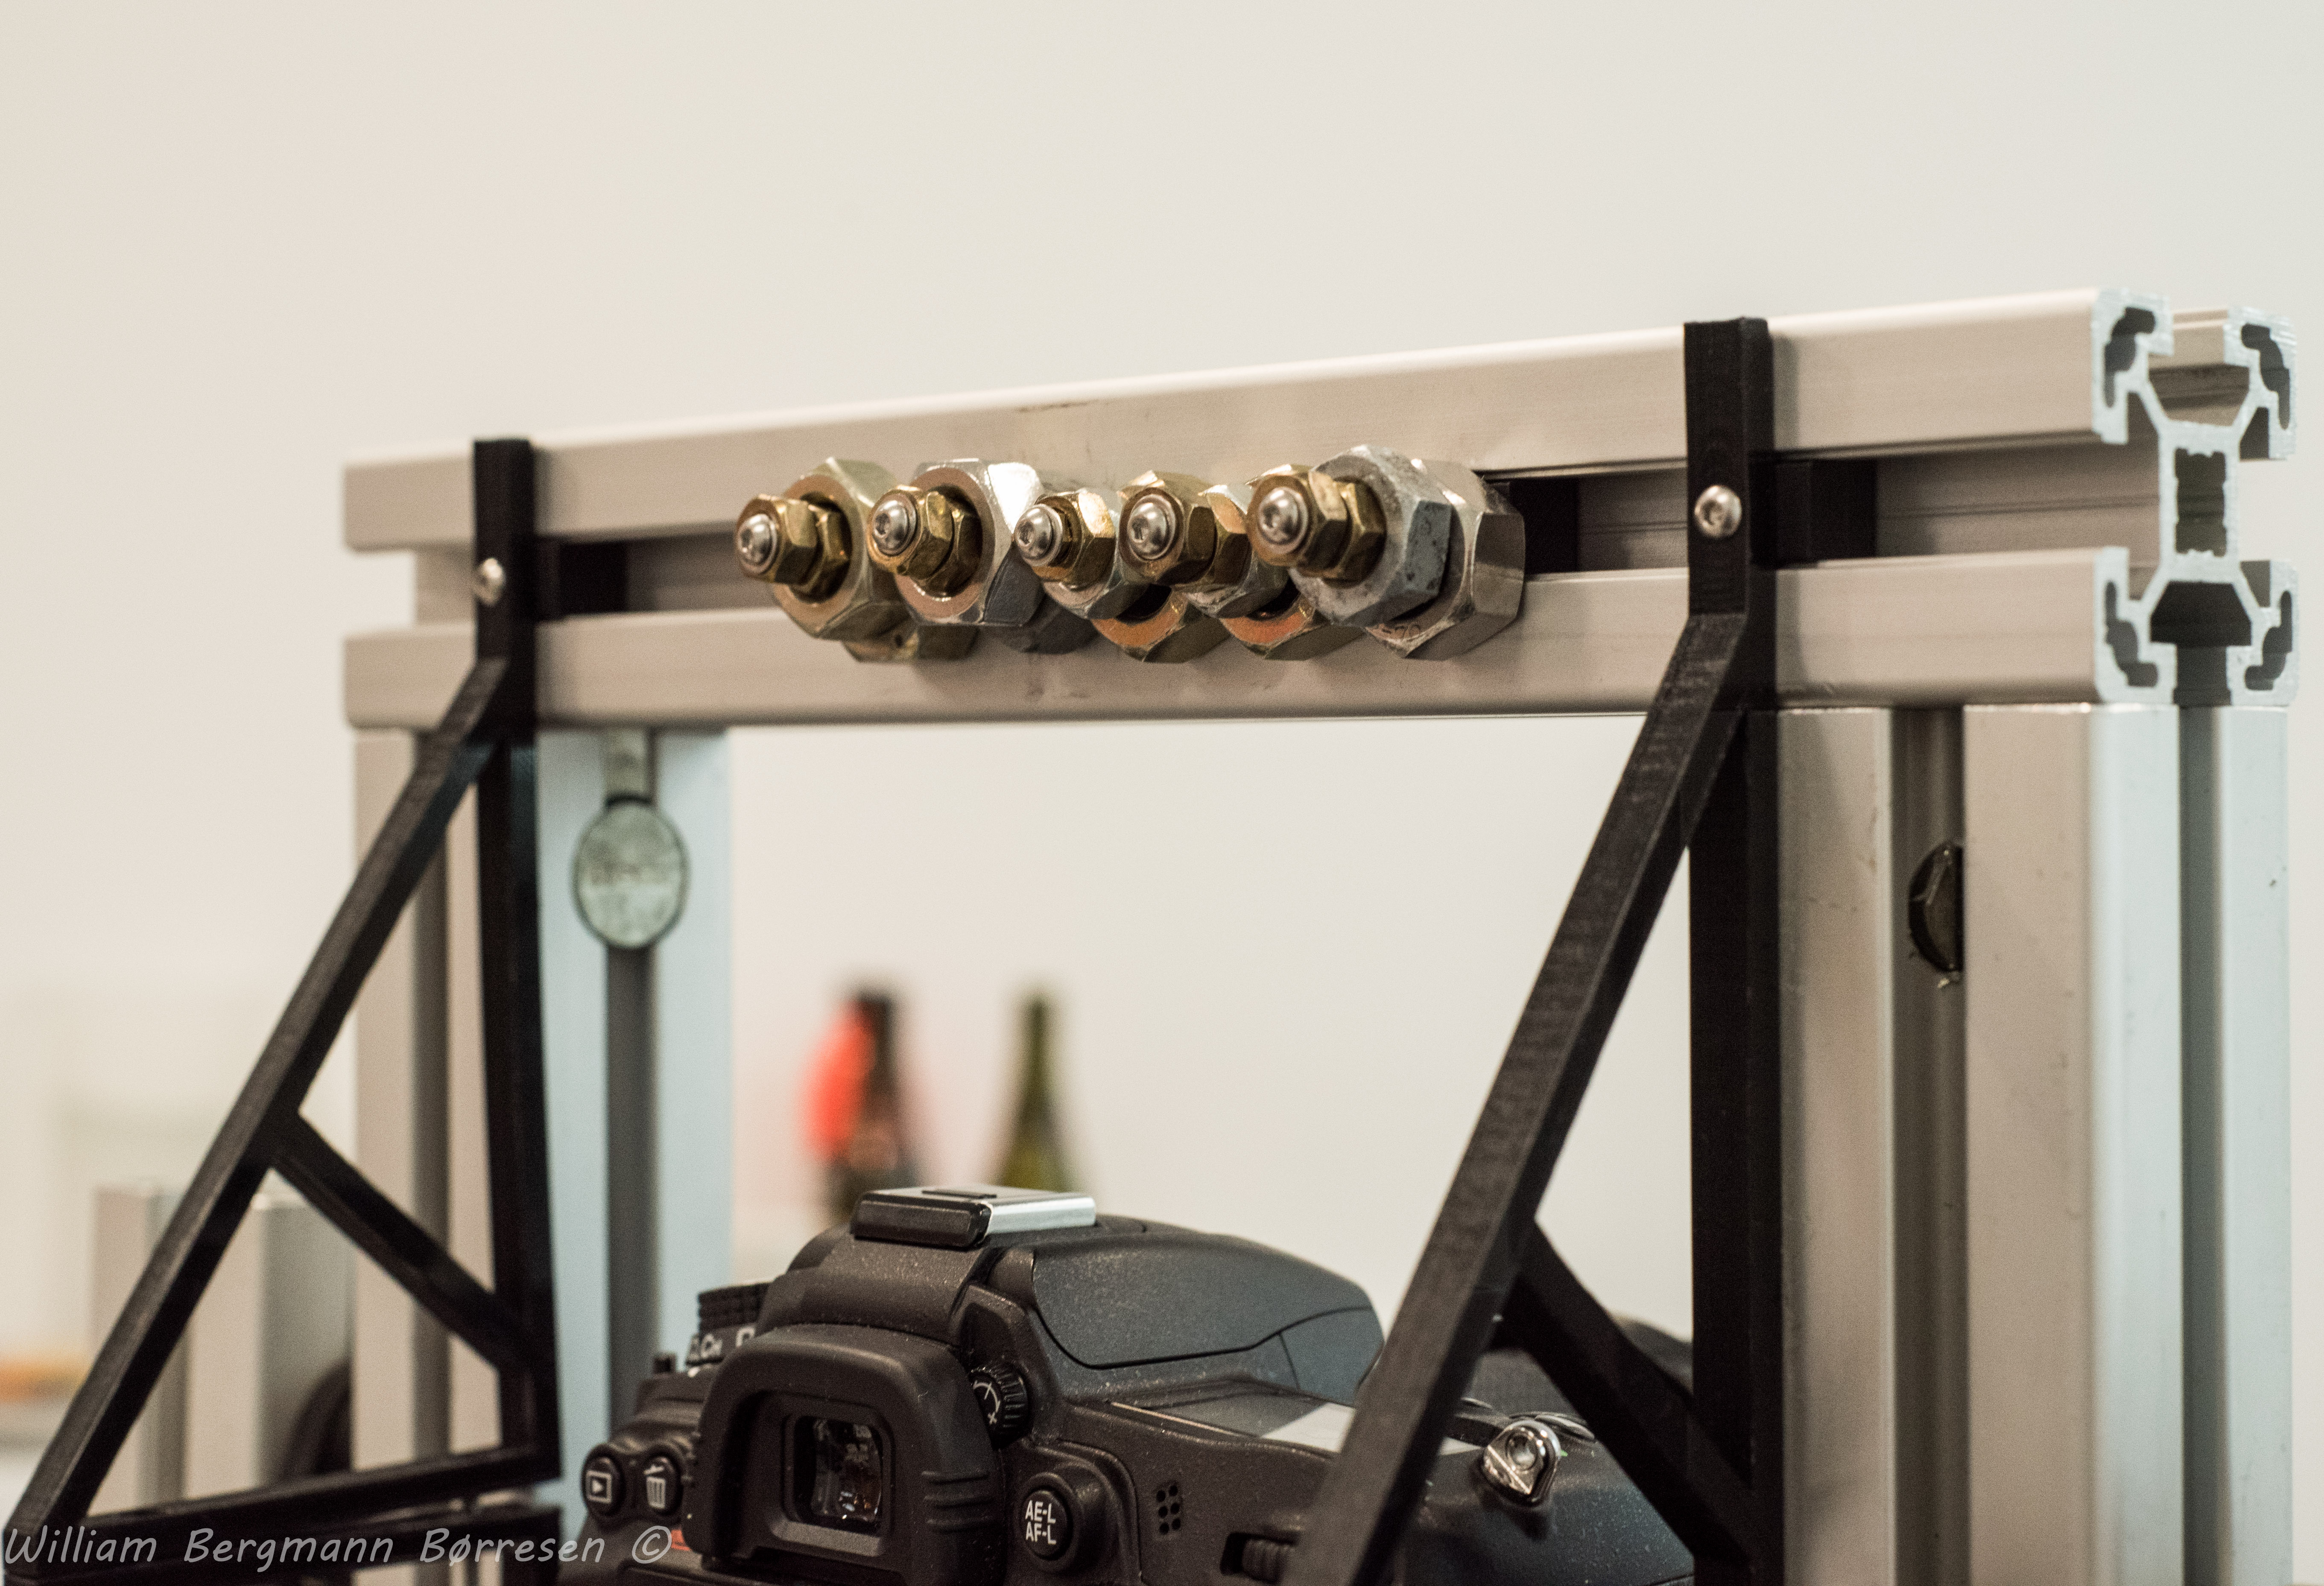
\includegraphics[scale=0.1]{Billeder/Afbalancering.jpg}
		\caption{Den tilføjede vægt, der opvejer misplaceringen af kameraet}
		\label{fig:Afbalancering}
	\end{center}
\end{figure}

Systemerne der er blevet udleveret, er rimelig godt afbalanceret, men efter der er blevet påmontere 1.4kg kamera er systemet ude af balance, dette kan ses på figur \ref{fig:Balanced_Response} hvor den orange graf er steprespons for systemet påmonteret kamera.\\

Kameraet vejer med ophænget 1.4kg, men er placeret en lille smule fra omdrejningspunktet, hvilket kunne ses ved at det altid faldt tilbage til et bestemt punkt når systemet blev frigjort fra motoren.
Ud fra den observation blev der placeredet vægt i den modsatte ende af tilt delen, til systemet ikke faldt tilbage til samme punkt hver gang. Efterfølgende er det blevet vejet til at være 0.17kg.

På figur \ref{fig:Afbalancering} kan man med den blå graf se stepresponset for tilt delen af systemet efter afbalanceringen. Hvis man sammenligner det med den røde graf på figur\ref{fig:Behandlet} så kan man se at systemet er tæt på at have samme steprespons som efter kameraet blev monteret.\\

%På figur \ref{fig:Balanced_Response} ses sammenligningen mellem tilt-systemet før og efter afbalancering. Det endelige resultat er stadigvæk ikke ideelt, men det er en del tættere på modellen.

\begin{figure}[!hb]
	\begin{center}
		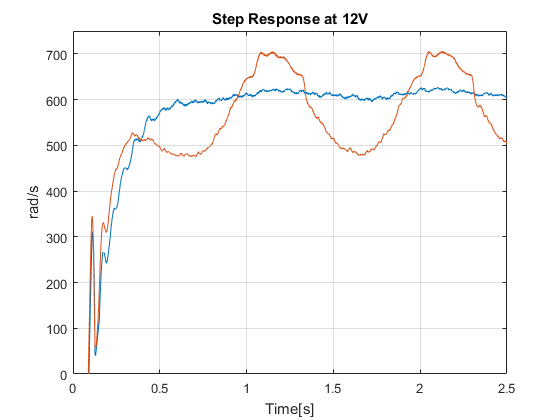
\includegraphics[width=0.8\textwidth]{Billeder/balanced_vs_unbalanced.png}
	\end{center}
	\caption{Orange graf Viser stepresponsen for tilt med kameraet monteret. Den blå graf Viser stepresponen for tilt med kamera og afbalancering monteret}
	\label{fig:Balanced_Response}
\end{figure}

\subsection{Omdrejningshastighed vs Duty Cycle}

En af antagelserne der bliver gjort i modellen af systemet, er at der findes en nogenlunde lineær sammenhæng imellem duty cycle og omdrejningshastigheden. For at påvise denne sammenhæng kan man plotte hastigheden, når motoren har nået steady state, ved forskellige duty cycles. 

Dette vises på figur \ref{fig:RPM_DC}, hvor man kan observere at stepresponet setler ved ca 50 rad/s højere for hver gange vi øger duty cyclen med 20 (på en skala fra 0-255).

Her kan man også se at hvis man plotter step responsen ved forskellige duty cycles (figur \ref{fig:RPM_DC}), kan det påvises at tidskonstanten forbliver nogenlunde konstant. 

\begin{figure}[!ht]
	\begin{center}
		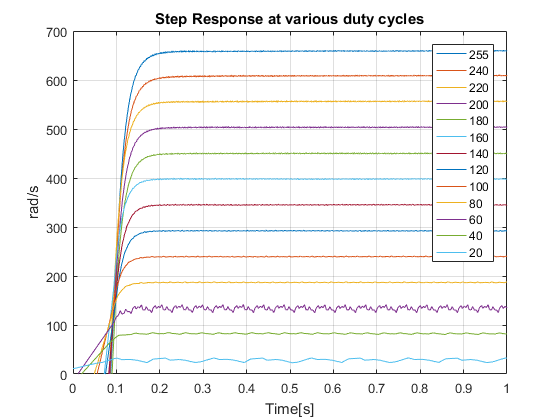
\includegraphics[width=0.8\textwidth]{Billeder/RPM_vs_DC.png}
	\end{center}
	\caption{Step Respons for tilt-rammen ved forskellige duty cycles}
	\label{fig:RPM_DC}
\end{figure}